\documentclass[border=3pt]{standalone}
% Preâmbulo compartilhado pelos diagramas TikZ da aula 8 de IHC (Design de IHC)
\usepackage[T1]{fontenc}
\usepackage[utf8]{inputenc}
\usepackage{lmodern}
\usepackage{amsmath}
\usepackage{xcolor}
\usepackage{tikz}
\usetikzlibrary{arrows.meta,angles,quotes,decorations.pathmorphing,decorations.pathreplacing,calc,
                positioning,shapes.geometric,shapes.misc,backgrounds,fit,
                math}

% Paleta (mesma dos SVGs originais)
% Paleta da disciplina de IHC: acento roxo (#755099), da capa do livro.
% (o nome "dblue" é mantido para não alterar todos os diagramas)
\definecolor{dblue}{HTML}{755099}
\definecolor{dorange}{HTML}{B3541E}
\definecolor{dgreen}{HTML}{4A7C59}
\definecolor{dred}{HTML}{9C4B4B}
\definecolor{dcream}{HTML}{F4F1EA}
\definecolor{dshade}{HTML}{DDD7C9}

% Função gaussiana (não normalizada por padrão de escala visual)
\pgfmathdeclarefunction{gauss}{3}{%
  \pgfmathparse{1/(#3*sqrt(2*pi))*exp(-((#1-#2)^2)/(2*#3^2))}%
}

% Estilos comuns (prefixo d... para não colidir com chaves internas do pgf)
\tikzset{
  >={Stealth[length=2mm]},
  dguide/.style={gray!55, dashed, line width=0.4pt},
  daxis/.style={gray!60, line width=0.7pt, ->},
  dbody/.style={fill=black!3, draw=black!80, line width=1pt},
  dacc/.style={draw=dblue, line width=1pt},
  dlbl/.style={black!55, font=\small},
  dsub/.style={black!45, font=\footnotesize},
  dstate/.style={circle, draw=black!80, fill=dcream, line width=1pt,
                 minimum size=17mm, font=\large, inner sep=1pt},
  dobs/.style={circle, draw=black!80, fill=dshade, line width=1pt,
               minimum size=14mm, font=\large, inner sep=1pt},
  dbox/.style={rounded corners=2pt, draw=black!80, fill=dcream, line width=1pt,
               align=center, inner sep=6pt},
  dop/.style={circle, draw=black!80, fill=white, line width=1pt,
              minimum size=6mm, inner sep=0pt, font=\small},
  dtrans/.style={->, dblue, line width=1pt},
  dmeas/.style={->, dorange, line width=1pt},
  dcurve/.style={line width=1pt, dblue},
  dcurveb/.style={line width=1.4pt, dorange},
}

\begin{document}
\hyphenpenalty=10000 \exhyphenpenalty=10000 \tolerance=9999 \emergencystretch=3em
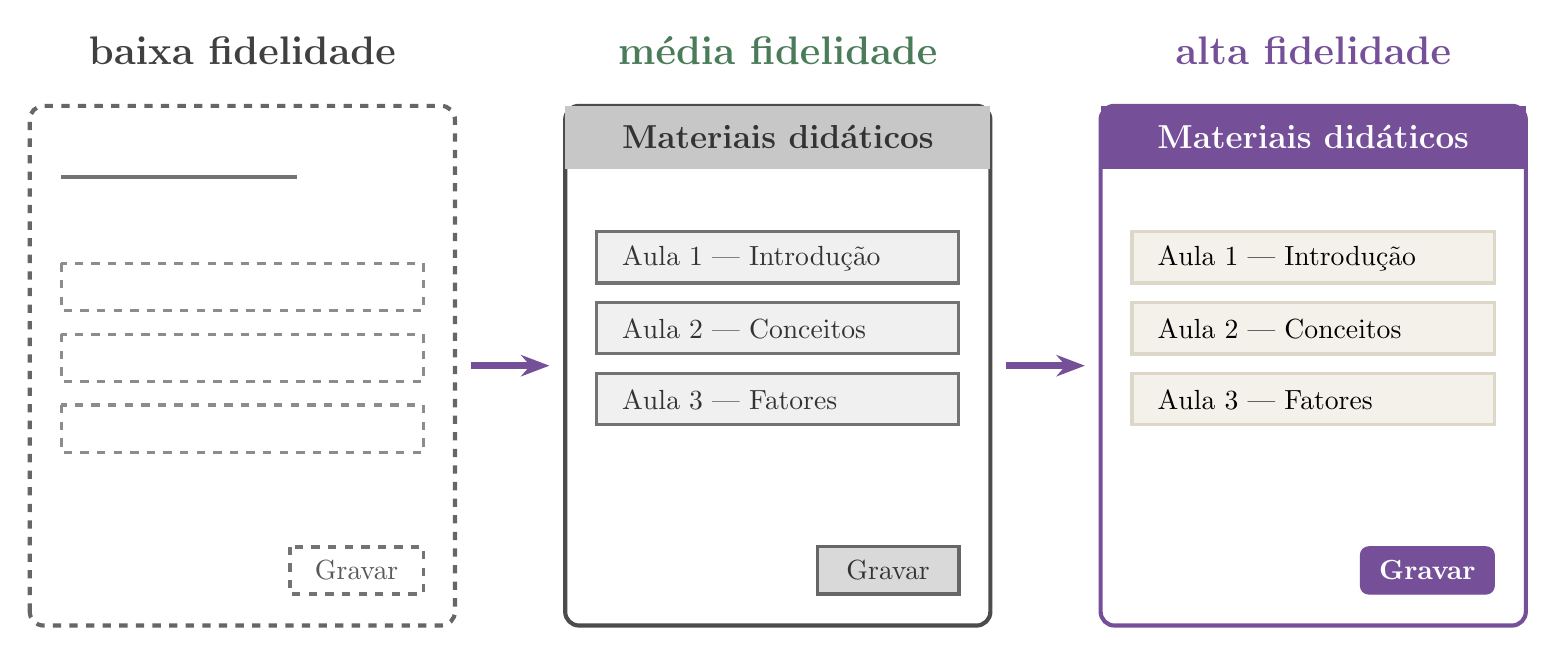
\begin{tikzpicture}[x=1cm,y=1cm]
\tikzset{legen/.style={font=\large, black!70, text width=5.6cm, align=center}}
% ---------- baixa ----------
\node[font=\Large\bfseries, black!75] at (2.7,9.0) {baixa fidelidade};
\draw[black!60, dashed, line width=1.5pt, rounded corners=5pt] (0,1.7) rectangle (5.4,8.3);
\draw[black!55, line width=1.4pt] (0.4,7.4) -- (3.4,7.4);
\foreach \y in {6.3,5.4,4.5} {\draw[black!45, dashed, line width=1.2pt] (0.4,\y) rectangle (5.0,\y-0.6);}
\draw[black!55, dashed, line width=1.4pt] (3.3,2.7) rectangle (5.0,2.1);
\node[font=\normalsize, black!65] at (4.15,2.4) {Gravar};
% ---------- média ----------
\node[font=\Large\bfseries, dgreen] at (9.5,9.0) {média fidelidade};
\draw[black!70, line width=1.5pt, rounded corners=5pt, fill=white] (6.8,1.7) rectangle (12.2,8.3);
\fill[black!22] (6.8,7.5) rectangle (12.2,8.3); \node[font=\large\bfseries, black!80] at (9.5,7.9) {Materiais didáticos};
\foreach \y/\t in {6.7/{Aula 1 --- Introdução},5.8/{Aula 2 --- Conceitos},4.9/{Aula 3 --- Fatores}} {
  \draw[black!55, fill=black!6, line width=1.1pt] (7.2,\y) rectangle (11.8,\y-0.65);
  \node[font=\normalsize, anchor=west, black!80] at (7.4,\y-0.33) {\t};}
\draw[black!60, fill=black!15, line width=1.2pt] (10.0,2.7) rectangle (11.8,2.1); \node[font=\normalsize, black!80] at (10.9,2.4) {Gravar};
% ---------- alta ----------
\node[font=\Large\bfseries, dblue] at (16.3,9.0) {alta fidelidade};
\draw[dblue, line width=1.5pt, rounded corners=5pt, fill=white] (13.6,1.7) rectangle (19.0,8.3);
\fill[dblue] (13.6,7.5) rectangle (19.0,8.3); \node[font=\large\bfseries, white] at (16.3,7.9) {Materiais didáticos};
\foreach \y/\t in {6.7/{Aula 1 --- Introdução},5.8/{Aula 2 --- Conceitos},4.9/{Aula 3 --- Fatores}} {
  \draw[dshade, fill=dcream, line width=1.2pt] (14.0,\y) rectangle (18.6,\y-0.65);
  \node[font=\normalsize, anchor=west] at (14.2,\y-0.33) {\t};}
\draw[dblue, fill=dblue, rounded corners=3pt] (16.9,2.7) rectangle (18.6,2.1); \node[font=\normalsize\bfseries, white] at (17.75,2.4) {Gravar};
% ---------- setas ----------
\draw[dtrans, line width=2.4pt, -{Stealth[length=3.6mm]}] (5.6,5.0) -- (6.6,5.0);
\draw[dtrans, line width=2.4pt, -{Stealth[length=3.6mm]}] (12.4,5.0) -- (13.4,5.0);
\end{tikzpicture}
\end{document}
